\documentclass[11pt]{article}

\usepackage[T1]{fontenc}
\usepackage{lmodern}
\usepackage[margin=0.90in]{geometry}
\usepackage{microtype}
\usepackage{amsmath,amssymb,amsthm,mathtools,mathrsfs}
\usepackage{booktabs,longtable,array,tabularx}
\usepackage{graphicx}
\usepackage{float}
\usepackage{xcolor}
\usepackage{enumitem}
\usepackage{fancyhdr}
\usepackage{hyperref}
\usepackage[nameinlink,noabbrev]{cleveref}
\usepackage{listings}
\usepackage{caption}
\usepackage{bm}
\usepackage{needspace}
\usepackage{placeins}
\usepackage{siunitx}

\graphicspath{{figures/}}
\allowdisplaybreaks
\sisetup{scientific-notation=true,round-mode=places,round-precision=4}

\hypersetup{
  pdftitle={Projector-Resolved Seed Calculus X},
  pdfauthor={Komorebi P.},
  pdfsubject={Universal residual seeds, deformation forests, directed transport, seed zeta functions, companion completion, compatible carriers, and finite occupancy},
  colorlinks=true,
  linkcolor=black,
  citecolor=black,
  urlcolor=black
}

\pagestyle{fancy}
\fancyhf{}
\fancyhead[L]{Projector-Resolved Seed Calculus X}
\fancyhead[R]{Komorebi P.}
\fancyfoot[C]{\thepage}
\setlength{\headheight}{14pt}

\newtheorem{theorem}{Theorem}[section]
\newtheorem{proposition}[theorem]{Proposition}
\newtheorem{lemma}[theorem]{Lemma}
\newtheorem{corollary}[theorem]{Corollary}
\theoremstyle{definition}
\newtheorem{definition}[theorem]{Definition}
\newtheorem{example}[theorem]{Example}
\newtheorem{conjecture}[theorem]{Conjecture}
\newtheorem{classicalinput}[theorem]{Classical Input}
\newtheorem{numericalcertificate}[theorem]{Numerical Certificate}
\theoremstyle{remark}
\newtheorem{remark}[theorem]{Remark}

\newcommand{\Ocal}{\mathcal O}
\newcommand{\mfrak}{\mathfrak m}
\newcommand{\F}{\mathbf F}
\newcommand{\Z}{\mathbf Z}
\newcommand{\Q}{\mathbf Q}
\newcommand{\C}{\mathbf C}
\newcommand{\Spf}{\operatorname{Spf}}
\newcommand{\Spec}{\operatorname{Spec}}
\newcommand{\GL}{\operatorname{GL}}
\newcommand{\Hom}{\operatorname{Hom}}
\newcommand{\End}{\operatorname{End}}
\newcommand{\Tr}{\operatorname{Tr}}
\newcommand{\Frob}{\operatorname{Frob}}
\newcommand{\WD}{\operatorname{WD}}
\newcommand{\HT}{\operatorname{HT}}
\newcommand{\ad}{\operatorname{ad}}
\newcommand{\red}{\operatorname{red}}
\newcommand{\Def}{\operatorname{Def}}
\newcommand{\rad}{\operatorname{rad}}
\newcommand{\srank}{\operatorname{srank}}
\newcommand{\Cl}{\operatorname{Cl}}
\newcommand{\SCC}{\operatorname{SCC}}
\newcommand{\rank}{\operatorname{rank}}
\newcommand{\im}{\operatorname{im}}
\newcommand{\coker}{\operatorname{coker}}
\newcommand{\id}{\operatorname{id}}
\newcommand{\Sys}{\mathscr S}
\newcommand{\Forest}{\mathfrak F}
\newcommand{\Compat}{\mathfrak C}
\newcommand{\Packet}{\mathfrak P}

\setlength{\parindent}{0pt}
\setlength{\parskip}{0.62em}
\setlist[itemize]{leftmargin=1.55em,itemsep=0.20em,topsep=0.30em}
\setlist[enumerate]{leftmargin=1.75em,itemsep=0.24em,topsep=0.32em}
\captionsetup{font=small,labelfont=bf}

\lstset{
  basicstyle=\ttfamily\scriptsize,
  breaklines=true,
  columns=fullflexible,
  frame=single,
  showstringspaces=false,
  tabsize=4,
  numbers=left,
  numberstyle=\tiny,
  xleftmargin=1.5em,
  framexleftmargin=1.2em
}

\title{\textbf{Projector-Resolved Seed Calculus X}\\[0.35em]
\large Universal Residual Seeds: Deformation Forests, Transport Categories, and System Completion}
\author{Komorebi P.}
\date{}

\begin{document}
\maketitle

\begin{abstract}
A residual representation is a genuine zeroth-order coordinate.  All positive-depth perturbations above it may fill its formal deformation neighborhood, but they cannot move into a different residual class.  This paper develops the corresponding universal object: a residual forest whose roots are residual representations, whose finite levels are lifts modulo powers of a uniformizer, and whose infinite branches are complete characteristic-zero objects.  We prove the residual partition, no-crossing, inverse-limit reconstruction, finite-branch compactness, exact smooth and singular branch counts, packet decomposition of tangent and obstruction cohomology, a directed minimum-seed theorem, rational seed-zeta formulas, and finite companion-forest completion.  The coefficient prime two is represented by a weighted forest in which characteristic-zero packets may merge modulo two and become visible only at later depth.  We then define a prime-independent system seed through a common Frobenius spine, prove a compatible-carrier summand theorem under finite Frobenius separation, and reduce finite occupancy in a fixed semisimple carrier to the nonnegative integer trace of an exact joint projector.  The paper does not prove that every admissible residual companion exists or that every finite Hecke packet is occupied.  Those two existence statements remain the exact horizontal boundary beyond vertical deformation theory.
\end{abstract}

\begin{center}
\fbox{\begin{minipage}{0.94\linewidth}
\textbf{Status of the paper.}  The formal, finite-graph, finite-complex, counting, compactness, compatible-carrier, and finite-projector statements are proved under their stated hypotheses.  Representability of Galois deformation functors and the identification of tangent and obstruction spaces with cohomology are classical inputs.  Universal residual companion existence, universal compatible-system completion, and universal automorphic occupancy are not proved.
\end{minipage}}
\end{center}

\tableofcontents
\newpage

\section{The universal seed at residual depth}

The earlier papers treat a seed as a primitive object together with an operator grammar, a packet system, a topology, and an exact reconstruction law.  In arithmetic deformation problems, the primitive coordinate has two layers:

\[
\boxed{
\text{residual root}
\quad+\quad
\text{positive-depth deformation coordinates}.
}
\]

The distinction is structural.  A correction divisible by the uniformizer changes higher digits but leaves the residual digit fixed.  Therefore the correct universal arithmetic seed cannot be one residual representation unless the admissible residual space has only one point.  It must contain every residual root and the complete formal neighborhood above each root.

Let \(\Ocal\) be a complete discrete valuation ring with uniformizer \(\varpi\), maximal ideal \((\varpi)\), residue field
\[
k=\Ocal/(\varpi),\qquad |k|=q,
\]
and fraction field \(K\).  Let \(\mathcal M\) be a moduli functor on complete local Noetherian \(\Ocal\)-algebras with residue field \(k\), equipped with a well-defined reduction map
\[
\red_A:\mathcal M(A)\longrightarrow \mathcal M(k).
\]
For a Galois representation this means either that a framed integral model has been fixed or that the residual semisimplified class is used.

\begin{definition}[Residual seed system]
For \(\bar x\in\mathcal M(k)\), define the residual fiber
\[
\mathcal M_{\bar x}(A)
=
\{x\in\mathcal M(A):\red_A(x)=\bar x\}.
\]
The point \(\bar x\) is the residual root.  The family of all nonempty fibers is the residual special fiber, and the formal deformation problems above them form the residual forest.
\end{definition}

For a Galois problem the principal example is
\[
\bar\rho:G_{F,S}\longrightarrow \GL_n(k),
\]
with a deformation functor \(\Def_{\bar\rho}\) cut out by a determinant and selected local conditions.

\begin{figure}[H]
\centering
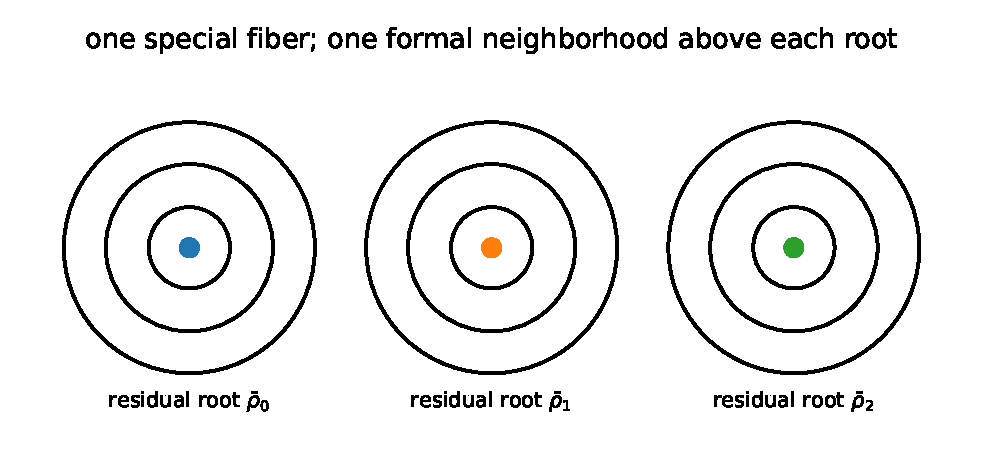
\includegraphics[width=0.87\linewidth]{01_residual_seed_architecture.pdf}
\caption{The universal residual seed is not one point.  It is the special fiber together with one complete formal neighborhood above each admissible root.}
\end{figure}

\subsection{What the paper is designed to separate}

Three statements are often compressed into one sentence even though they have different logical content.

\begin{enumerate}
\item \textbf{Vertical completeness:} every compatible perturbation stream above a fixed root reconstructs a point of its complete deformation space.
\item \textbf{Horizontal companion existence:} every required residual root, including roots at other coefficient primes, actually exists.
\item \textbf{Occupancy:} the resulting arithmetic packet occurs in a nonzero global carrier of the required type.
\end{enumerate}

The first belongs to deformation and inverse-limit theory.  The second is a residual companion problem.  The third is an arithmetic or automorphic nonvanishing problem.  Neither of the last two follows from arbitrarily deep perturbation above one already occupied root.

\section{Residual partition and no crossing}

\begin{theorem}[Residual partition]
For every coefficient algebra \(A\),
\[
\boxed{
\mathcal M(A)
=
\bigsqcup_{\bar x\in\mathcal M(k)}
\mathcal M_{\bar x}(A).
}
\]
\end{theorem}

\begin{proof}
Every \(A\)-valued object has one reduced object \(\red_A(x)\in\mathcal M(k)\), so the union is exhaustive.  Two distinct fibers cannot intersect because an object cannot have two different reductions.  Hence the union is disjoint.
\end{proof}

\begin{theorem}[No crossing under positive-depth perturbation]
Suppose \(x,y\in\mathcal M(\Ocal)\) are related by a deformation operation that is congruent to the identity modulo \(\varpi\).  Then
\[
\red(x)=\red(y).
\]
Every finite or infinite composition of such positive-depth operations remains in one residual fiber.
\end{theorem}

\begin{proof}
A correction in \(\varpi\Ocal\) vanishes after reduction modulo \(\varpi\).  Thus one operation preserves the residual root.  Induction proves the finite statement.  Every finite prefix of an infinite perturbation stream has the same reduction, and completeness does not alter the first digit.
\end{proof}

\begin{corollary}[Zeroth-order obstruction]
If two admissible objects have different residual roots, no sequence of genuinely positive-depth perturbations beginning at one can reach the other.  A horizontal transport between their roots is a zeroth-order operation, not a deeper lift.
\end{corollary}

\begin{figure}[H]
\centering
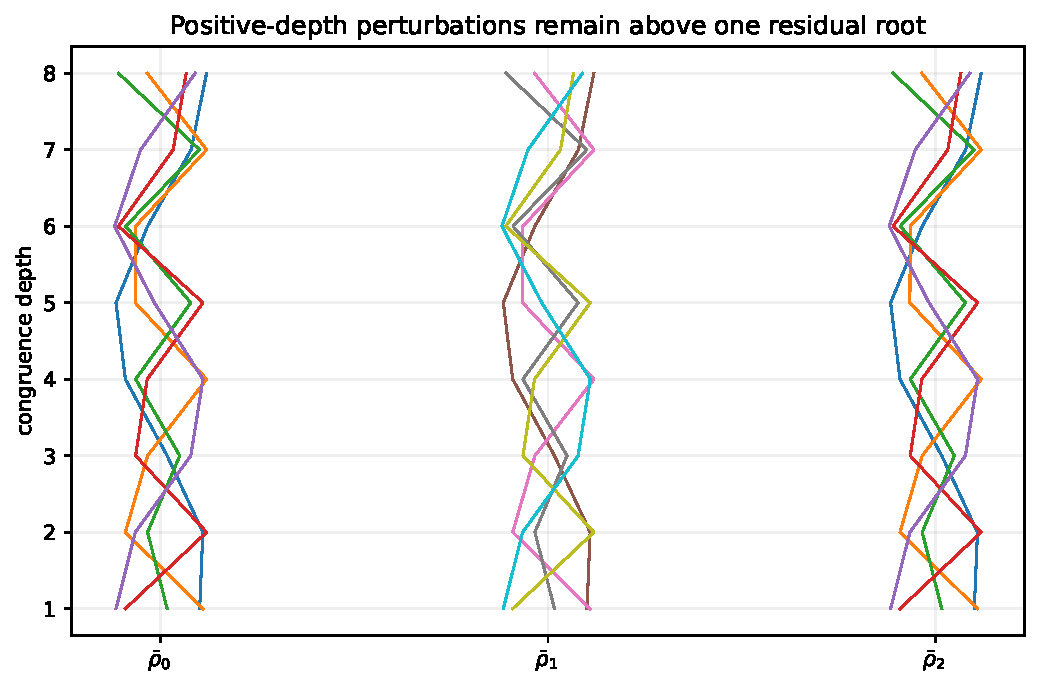
\includegraphics[width=0.95\linewidth]{03_no_crossing_branches.pdf}
\caption{Each perturbation stream remains above its initial residual root.  Refinement adds digits vertically; it does not move a branch horizontally.}
\end{figure}

\begin{numericalcertificate}[Exact residual partition]
The finite implementation partitions the integers \(0,\ldots,8\) into the three classes modulo \(3\):
\[
\{0,3,6\},\qquad \{1,4,7\},\qquad \{2,5,8\}.
\]
Every tested correction of the form \(x\mapsto x+p h\) preserves the residual class exactly.
\end{numericalcertificate}

\section{Lift forests and inverse-limit reconstruction}

Fix \(\bar x\in\mathcal M(k)\).  For \(m\ge1\), set
\[
X_m(\bar x)=\mathcal M_{\bar x}(\Ocal/\varpi^m).
\]
Reduction gives transition maps
\[
r_{m+1,m}:X_{m+1}(\bar x)\longrightarrow X_m(\bar x).
\]
A compatible branch is a sequence \((x_m)_{m\ge1}\) satisfying
\[
r_{m+1,m}(x_{m+1})=x_m.
\]

\begin{classicalinput}[Represented complete deformation problems]
When a deformation functor is represented by a complete local ring \(R_{\bar x}\), its \(\Ocal\)-valued points are continuous local maps \(R_{\bar x}\to\Ocal\).  Completeness identifies such maps with compatible maps to every quotient \(\Ocal/\varpi^m\).
\end{classicalinput}

\begin{theorem}[Formal inverse-limit reconstruction]
Assume \(\mathcal M_{\bar x}\) is represented by a complete local \(\Ocal\)-algebra \(R_{\bar x}\).  Then reduction induces a natural bijection
\[
\boxed{
\mathcal M_{\bar x}(\Ocal)
\cong
\varprojlim_m
\mathcal M_{\bar x}(\Ocal/\varpi^m).
}
\]
\end{theorem}

\begin{proof}
A continuous local homomorphism \(R_{\bar x}\to\Ocal\) reduces to a compatible family of homomorphisms into \(\Ocal/\varpi^m\).  Conversely, compatible finite-level maps determine a map
\[
R_{\bar x}\longrightarrow\varprojlim_m\Ocal/\varpi^m\cong\Ocal.
\]
The two constructions are inverse because equality in a separated complete ring is detected modulo every power of its maximal ideal.
\end{proof}

\begin{theorem}[Finite-branch compactness]
Suppose every \(X_m(\bar x)\) is finite and nonempty and every node has finitely many children.  Then the lift tree above \(\bar x\) contains an infinite compatible branch.
\end{theorem}

\begin{proof}
The tree is infinite because it has a nonempty level at every depth, and it is finitely branching by hypothesis.  K\"onig's lemma gives an infinite path.  The edge relation is reduction, so that path is a compatible branch.
\end{proof}

Surjectivity of every transition map is sufficient but not necessary.  Finite branching and nonempty arbitrarily deep levels are the compactness mechanism.

\begin{proposition}[Smooth formal branch count]
If
\[
R_{\bar x}\cong\Ocal[[t_1,\ldots,t_d]],
\]
then
\[
\boxed{
\#X_m(\bar x)=q^{d(m-1)}.
}
\]
Every \(\Ocal\)-valued branch is encoded by \(d\) positive-depth digit streams
\[
t_i=a_{i,1}\varpi+a_{i,2}\varpi^2+\cdots,
\qquad a_{i,j}\in k.
\]
\end{proposition}

\begin{proof}
A local map sends each parameter into \(\varpi\Ocal/\varpi^m\), a set of size \(q^{m-1}\).  The \(d\) choices are independent, giving \(q^{d(m-1)}\).  Passing to the inverse limit writes each chosen value in its unique digit expansion.
\end{proof}

\begin{figure}[H]
\centering
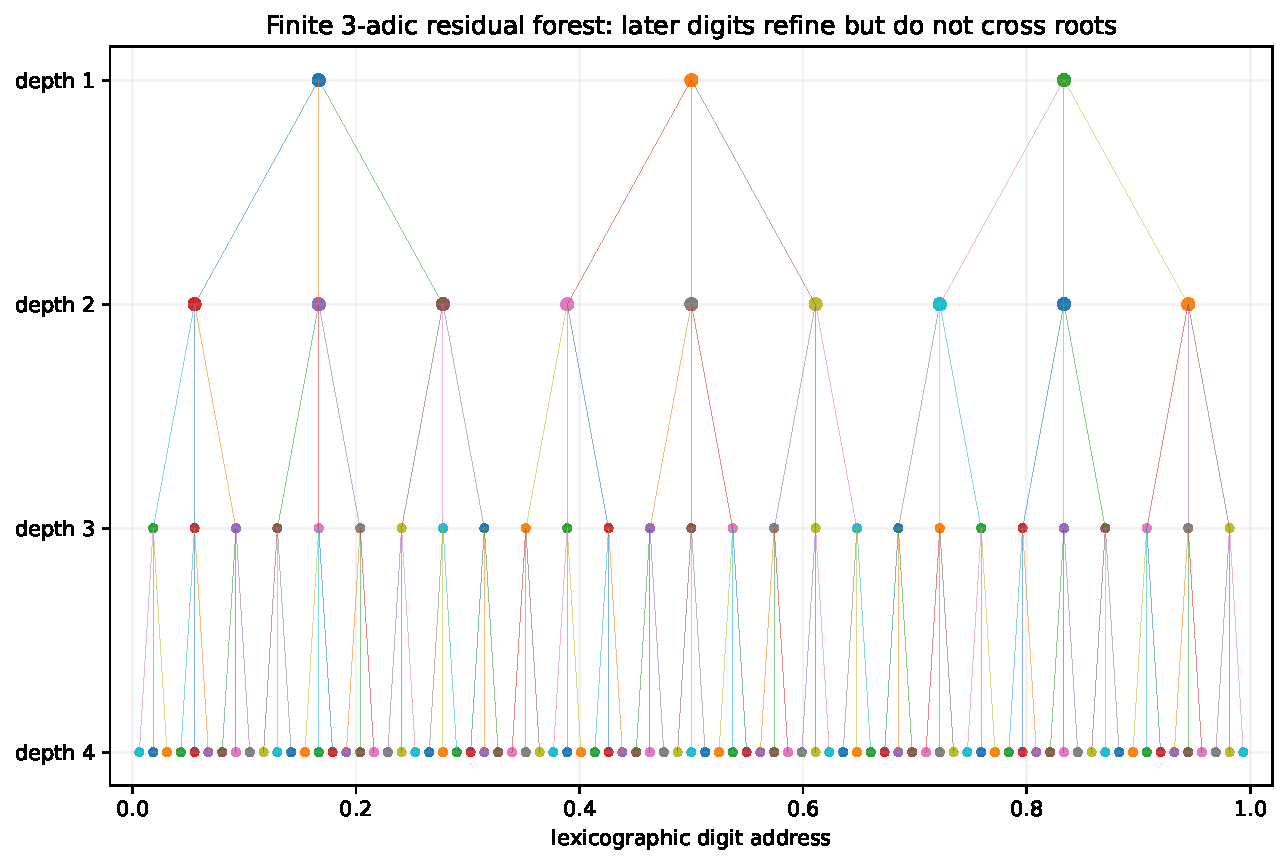
\includegraphics[width=0.94\linewidth]{02_residual_digit_forest.pdf}
\caption{The first four levels of a full \(3\)-adic digit forest.  A path is a compatible finite-depth perturbation stream.}
\end{figure}

\begin{figure}[H]
\centering
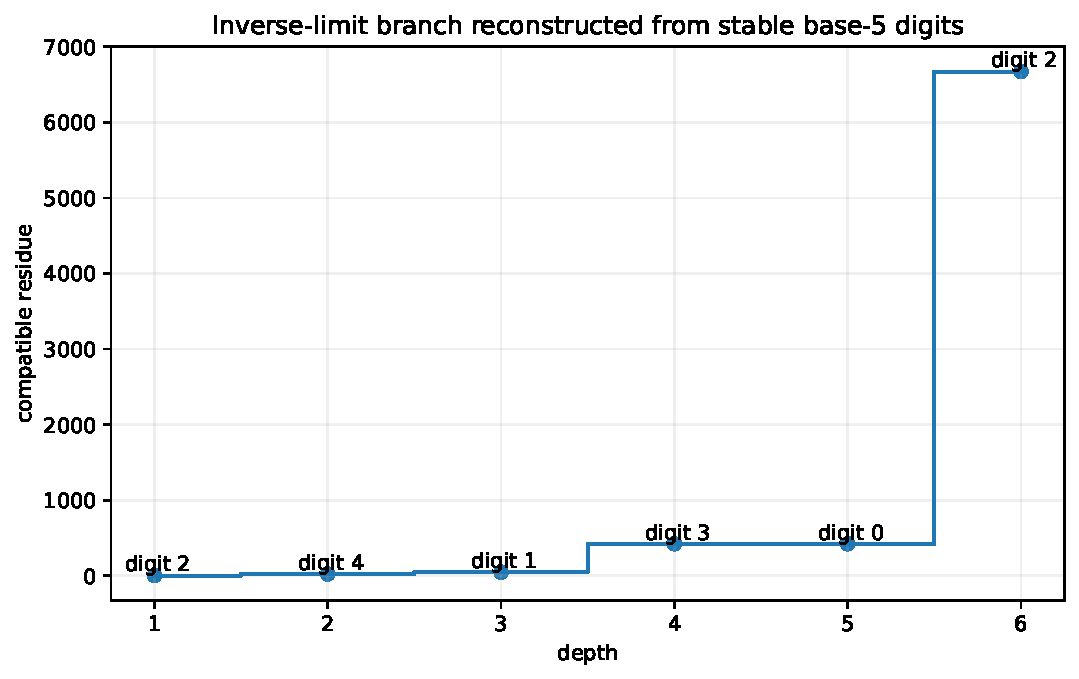
\includegraphics[width=0.82\linewidth]{04_inverse_limit_digits.pdf}
\caption{A compatible base-five residue tower reconstructs the digit stream \((2,4,1,3,0,2)\).}
\end{figure}

\section{Tangent and obstruction packets}

For a residual representation \(\bar\rho\), first-order deformations and lifting obstructions are classically controlled by cohomology of the adjoint module.  The projector calculus does not replace that theory.  It resolves the controlling complex into invariant packets when suitable projectors exist.

\begin{classicalinput}[Tangent and obstruction spaces]
For a framed representation problem, first-order lifts are described by \(Z^1(G,\ad\bar\rho)\).  For an unframed Schur problem, tangent directions are described by \(H^1(G,\ad\bar\rho)\).  Relations in a presentation of a deformation ring map into \(H^2(G,\ad\bar\rho)\), which contains the obstruction classes.
\end{classicalinput}

Let
\[
C^0\xrightarrow{d_0}C^1\xrightarrow{d_1}C^2\xrightarrow{}\cdots
\]
be a cochain complex over a field.  Suppose a finite family of projectors \(P_j^r:C^r\to C^r\) satisfies
\[
\sum_jP_j^r=I,
\qquad
P_i^rP_j^r=\delta_{ij}P_j^r,
\qquad
d_rP_j^r=P_j^{r+1}d_r.
\]

\begin{theorem}[Cohomology packet decomposition]
Under these hypotheses, each packet is a subcomplex and
\[
\boxed{
H^r(C^\bullet)
\cong
\bigoplus_jH^r(P_jC^\bullet).
}
\]
In particular,
\[
H^1=\bigoplus_jH^1_j,
\qquad
H^2=\bigoplus_jH^2_j,
\]
so tangent and obstruction spaces reconstruct exactly from their packet components.
\end{theorem}

\begin{proof}
Commutation with the differential makes \(P_jC^\bullet\) a subcomplex.  The direct-sum decomposition of each cochain space carries cocycles and coboundaries into direct sums:
\[
\ker d_r=\bigoplus_j\ker(d_r|_{P_jC^r}),
\qquad
\im d_{r-1}=\bigoplus_j\im(d_{r-1}|_{P_jC^{r-1}}).
\]
Taking the quotient gives the claimed decomposition.
\end{proof}

\begin{remark}[Odd and dyadic nonlinear equations]
At odd residue characteristic, a differential graded Lie model may be written in Maurer--Cartan form
\[
d\eta+\frac12[\eta,\eta]=0,
\]
and a cyclic grading converts this into exact packet convolutions.  At residue characteristic two, division by \(2\) is not integral.  A quadratic or divided-square refinement must be retained.  This is one reason the dyadic residual forest is weighted rather than obtained by formal substitution into the odd-prime formulas.
\end{remark}

\begin{numericalcertificate}[Finite packet complex]
The exact modular test uses two invariant subcomplexes over \(\F_5\).  Their cohomology dimensions are
\[
(0,0,0),
\qquad
(1,2,1),
\]
and the reconstructed total is
\[
\dim(H^0,H^1,H^2)=(1,2,1).
\]
The packet-sum residual is zero.
\end{numericalcertificate}

\begin{figure}[H]
\centering
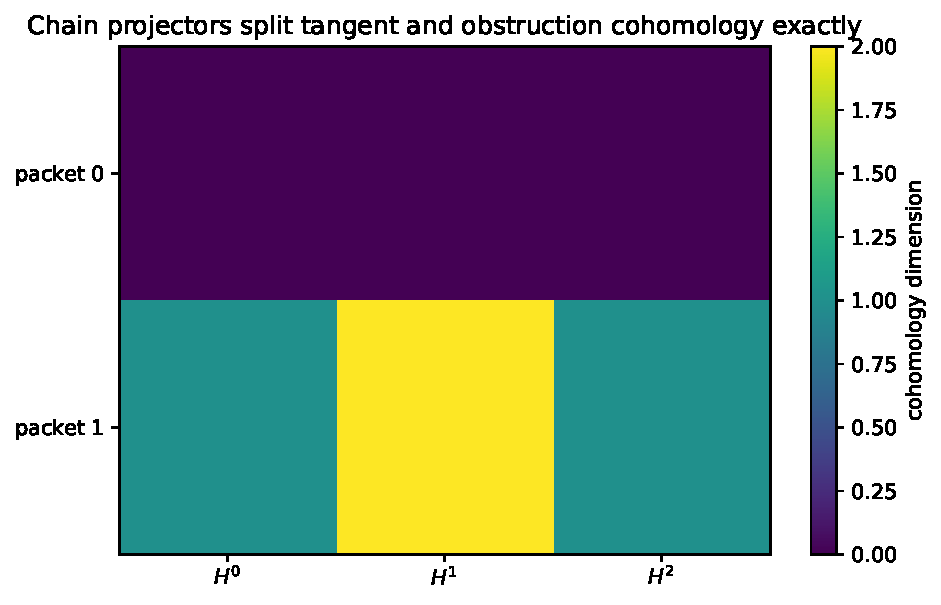
\includegraphics[width=0.78\linewidth]{11_tangent_obstruction_packets.pdf}
\caption{A finite chain-projector model.  Tangent and obstruction dimensions are carried by one packet and reconstruct exactly.}
\end{figure}

\section{The weighted dyadic residual forest}

At an odd prime, distinct sign characters remain distinct in the residue field.  At the coefficient prime two,
\[
1\equiv-1\pmod2.
\]
Thus distinct characteristic-zero packets can share one residual root and separate only after more precision is retained.

\begin{definition}[Visibility weight]
For two integral packet coordinates \(a,b\in\Ocal\), define their separation depth
\[
w(a,b)=\min\{m\ge1:a\not\equiv b\pmod{\varpi^m}\},
\]
when such an \(m\) exists.  A dyadic packet decomposition is weighted by these first visibility depths and by the valuations of any denominators required by its rational projectors.
\end{definition}

\begin{example}[The two sign branches]
The characters \(\chi_+(g)=1\) and \(\chi_-(g)=-1\) have the same reduction modulo \(2\), but
\[
1\not\equiv-1\pmod4.
\]
Their first separation depth is therefore \(2\).  One mod-two root contains two branches that become distinct at the next level.
\end{example}

\begin{figure}[H]
\centering
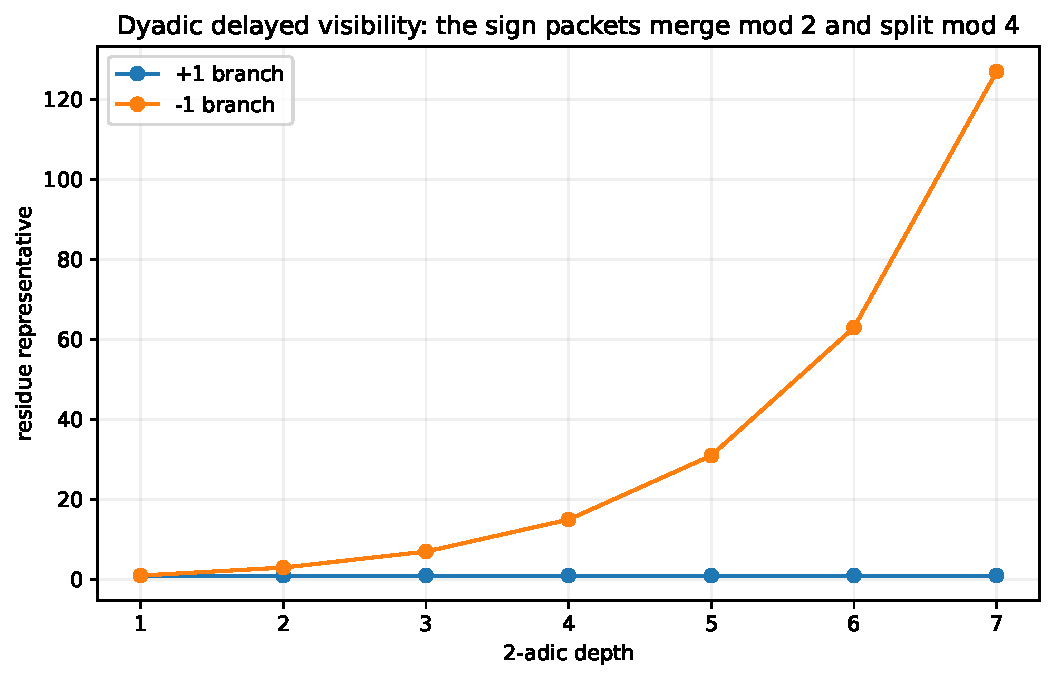
\includegraphics[width=0.82\linewidth]{05_dyadic_delayed_separation.pdf}
\caption{The sign packets merge at residual depth and separate at depth two.  This is a genuine change in integral coordinates, not a numerical plotting effect.}
\end{figure}

A simple weighted formal model already captures delayed visibility.  Let \(w_i\ge1\) and constrain
\[
t_i\in\varpi^{w_i}\Ocal/\varpi^m.
\]
Then coordinate \(i\) is invisible until \(m>w_i\).

\begin{proposition}[Weighted smooth-chart count]
For weights \(\bm w=(w_1,\ldots,w_d)\),
\[
\boxed{
N_{\bm w}(m)
=
q^{\sum_{i=1}^d\max(m-w_i,0)}.
}
\]
\end{proposition}

\begin{proof}
The ideal \(\varpi^{w_i}\Ocal/\varpi^m\) has one element when \(m\le w_i\), and \(q^{m-w_i}\) elements when \(m>w_i\).  Multiplying the independent coordinate counts gives the formula.
\end{proof}

This model does not assert that every dyadic Galois deformation ring is a weighted formal ball.  It gives the exact local counting law once such weighted coordinates or a Smith-normal-form chart have been proved.

\begin{figure}[H]
\centering
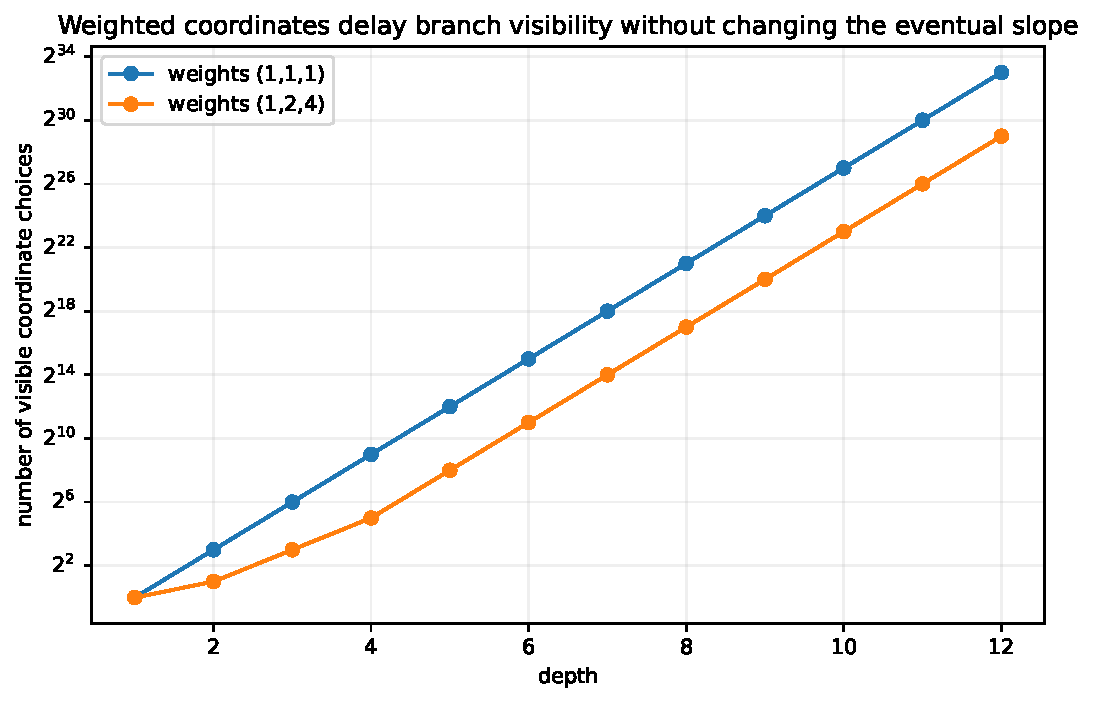
\includegraphics[width=0.82\linewidth]{07_weighted_formal_chart.pdf}
\caption{Weights delay finite-depth visibility.  Once all coordinates are active, the asymptotic slope equals the ordinary formal dimension.}
\end{figure}

\section{Seed zeta functions and branching dimensions}

Finite-depth counts record more than the existence of a branch.  They distinguish smooth, weighted, and singular local geometry.

\begin{definition}[Seed zeta function]
For a residual root \(\bar x\) with finite levels, define
\[
\boxed{
Z_{\bar x}(T)
=
\sum_{m\ge1}\#X_m(\bar x)T^m.
}
\]
When a weighted chart is specified, write \(Z_{\bm w}(T)\).
\end{definition}

\begin{theorem}[Smooth seed zeta function]
For a smooth formal component of dimension \(d\),
\[
\boxed{
Z_d(T)=\frac{T}{1-q^dT}.
}
\]
\end{theorem}

\begin{proof}
Insert \(\#X_m=q^{d(m-1)}\) and sum the geometric series.
\end{proof}

\begin{theorem}[Weighted seed zeta function]
Let \(1\le w_1\le\cdots\le w_d\), put \(W=\sum_iw_i\), and let
\[
a_m=q^{\sum_i\max(m-w_i,0)}.
\]
Then
\[
\boxed{
Z_{\bm w}(T)
=
\sum_{m=1}^{w_d}a_mT^m
+
q^{-W}\frac{(q^dT)^{w_d+1}}{1-q^dT}.
}
\]
In particular, every weighted smooth chart has a rational seed zeta function.
\end{theorem}

\begin{proof}
The finite sum records the depths before all coordinates are active.  For \(m\ge w_d+1\),
\[
a_m=q^{dm-W},
\]
so the remaining terms form one geometric series.
\end{proof}

\begin{theorem}[Singular power seed]
In \(\Ocal/\varpi^m\), the equation
\[
x^e=0
\]
has exactly
\[
\boxed{
q^{m-\lceil m/e\rceil}
}
\]
solutions.  Its seed zeta function is
\[
\boxed{
Z_e(T)
=
\frac{\sum_{r=1}^{e}q^{r-1}T^r}
{1-q^{e-1}T^e}.
}
\]
\end{theorem}

\begin{proof}
The congruence is equivalent to
\[
e\,v_\varpi(x)\ge m,
\]
so \(x\) must lie in \(\varpi^{\lceil m/e\rceil}\Ocal/\varpi^m\), which has the stated cardinality.  Write \(m=ek+r\), \(1\le r\le e\).  The exponent becomes \((e-1)k+r-1\).  Summing over \(k\ge0\) and \(1\le r\le e\) gives the rational expression.
\end{proof}

\begin{definition}[Branching dimension]
When the limit exists, define
\[
\dim_{\mathrm{seed}}(\bar x)
=
\lim_{m\to\infty}
\frac{\log_q\#X_m(\bar x)}{m}.
\]
A limsup may be used in general.
\end{definition}

\begin{corollary}[Fractional singular dimension]
For \(x^e=0\),
\[
\boxed{
\dim_{\mathrm{seed}}=1-\frac1e.
}
\]
In particular, \(x^2=0\) has branching dimension \(1/2\).
\end{corollary}

\begin{figure}[H]
\centering
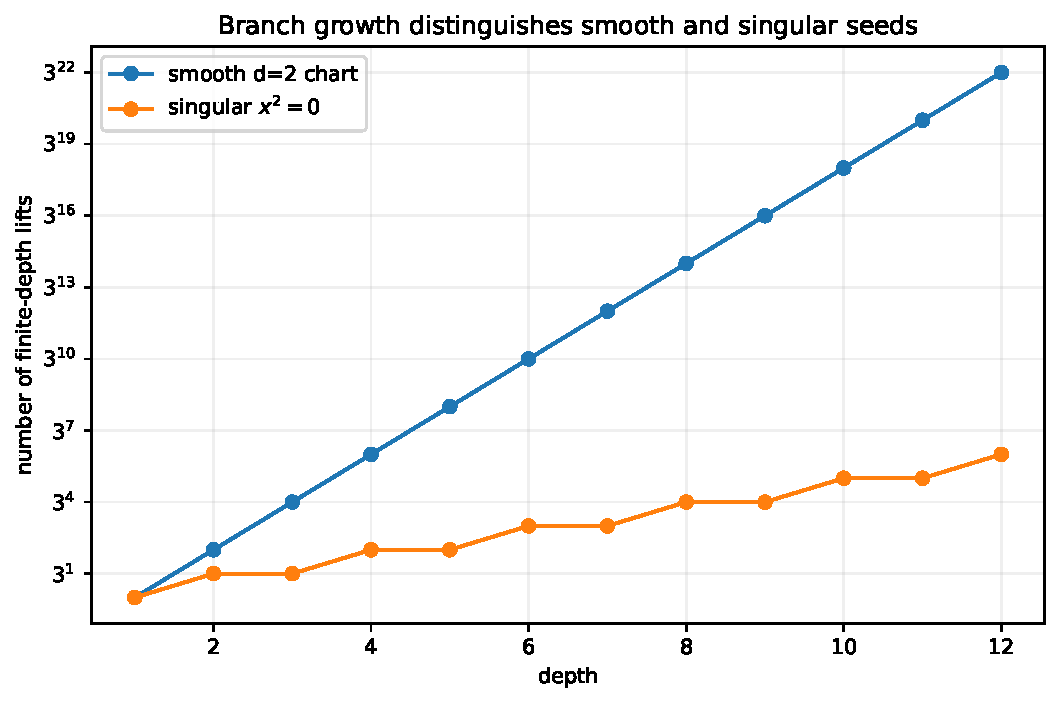
\includegraphics[width=0.83\linewidth]{06_smooth_singular_counts.pdf}
\caption{A smooth two-dimensional formal chart and the singular equation \(x^2=0\) have visibly different exponential growth.}
\end{figure}

\begin{figure}[H]
\centering
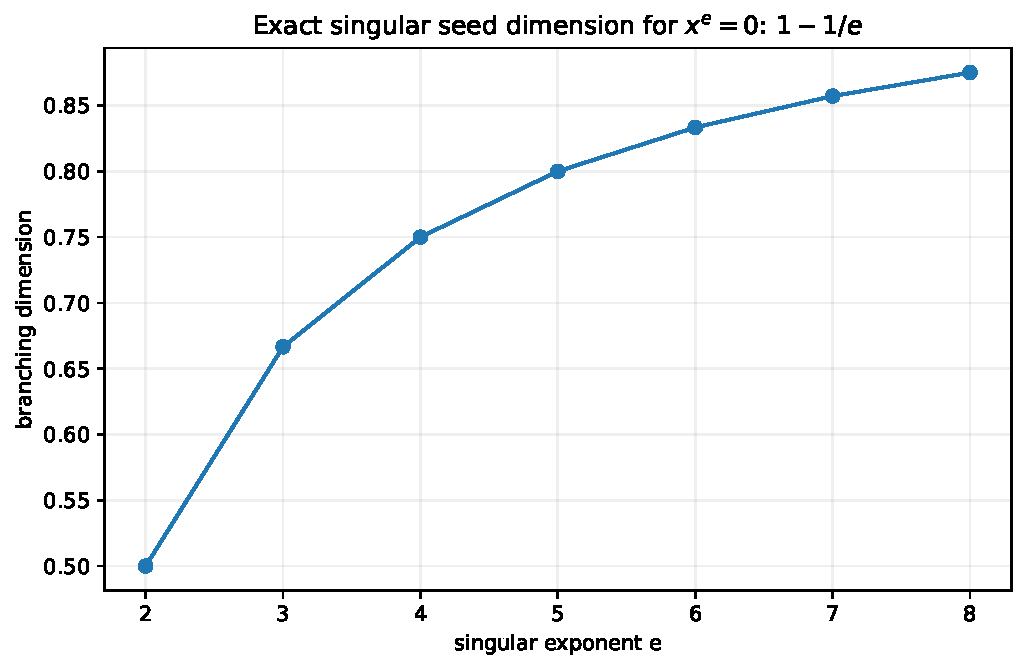
\includegraphics[width=0.78\linewidth]{08_fractional_seed_dimension.pdf}
\caption{The finite-depth branching dimension of \(x^e=0\) is \(1-1/e\), giving a family of fractional local growth exponents.}
\end{figure}

\section{Residual transport categories}

Vertical lifting never changes a residual root.  Horizontal coverage requires operations whose residual effect is not congruent to the identity.  Examples that may define such transports include twisting, duality, restriction, induction, tensor product, symmetric powers, exterior powers, and functorial transfer.  The word ``may'' is essential: each operation must preserve the deformation conditions and the realization statement being transported.

\begin{definition}[Admissible residual transport]
An admissible transport from \(\bar\rho\) to \(\bar\rho'\) consists of
\[
\mathcal T:\bar\rho\longmapsto\bar\rho'
\]
together with natural maps
\[
\mathcal T_A:\Def_{\bar\rho}(A)\longrightarrow\Def_{\bar\rho'}(A)
\]
for every coefficient algebra \(A\), compatible with base change and reduction.  When the transport is reversible, it is an isomorphism in the residual transport groupoid.  One-way operations give a directed category.
\end{definition}

For a finite collection of roots, record a directed edge \(u\to v\) whenever occupancy or the relevant property is known to propagate from \(u\) to \(v\).

\begin{definition}[Directed seed rank]
For a directed transport graph \(G\), define
\[
\srank_G
=
\min\{|S|:\Cl_G(S)=V(G)\},
\]
where \(\Cl_G(S)\) is the set of vertices reachable from \(S\).
\end{definition}

\begin{theorem}[Directed minimum-seed theorem]
Let \(G\) be a finite directed graph.  Collapse every strongly connected component to one vertex, obtaining the condensation DAG.  Then
\[
\boxed{
\srank_G
=
\#\{\text{source strongly connected components of }G\}.
}
\]
One representative from each source component is a minimum seed set.
\end{theorem}

\begin{proof}
Every vertex of a finite DAG is reachable from a source, so one seed in each source component reaches the entire condensation graph.  Within a strongly connected component, one vertex reaches every other.  Hence the source representatives are sufficient.

Conversely, a source component has no incoming edge from another component.  It cannot be reached from a seed outside itself, so every generating seed set must meet it.  Therefore the number of source components is also a lower bound.
\end{proof}

For reversible transports the condensation has one vertex per connected component, recovering the undirected minimum-seed theorem.

\begin{figure}[H]
\centering
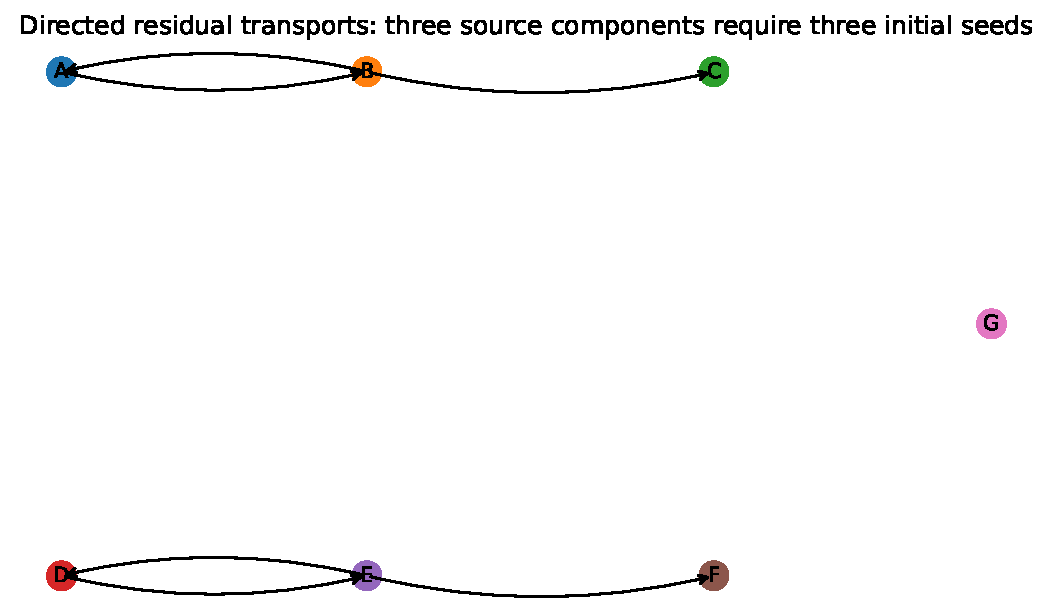
\includegraphics[width=0.91\linewidth]{09_directed_transport_graph.pdf}
\caption{A finite directed transport model.  The components \(\{A,B\}\), \(\{D,E\}\), and \(\{G\}\) are sources; \(C\) and \(F\) are reached downstream.}
\label{fig:transport-graph}
\end{figure}

\begin{figure}[H]
\centering
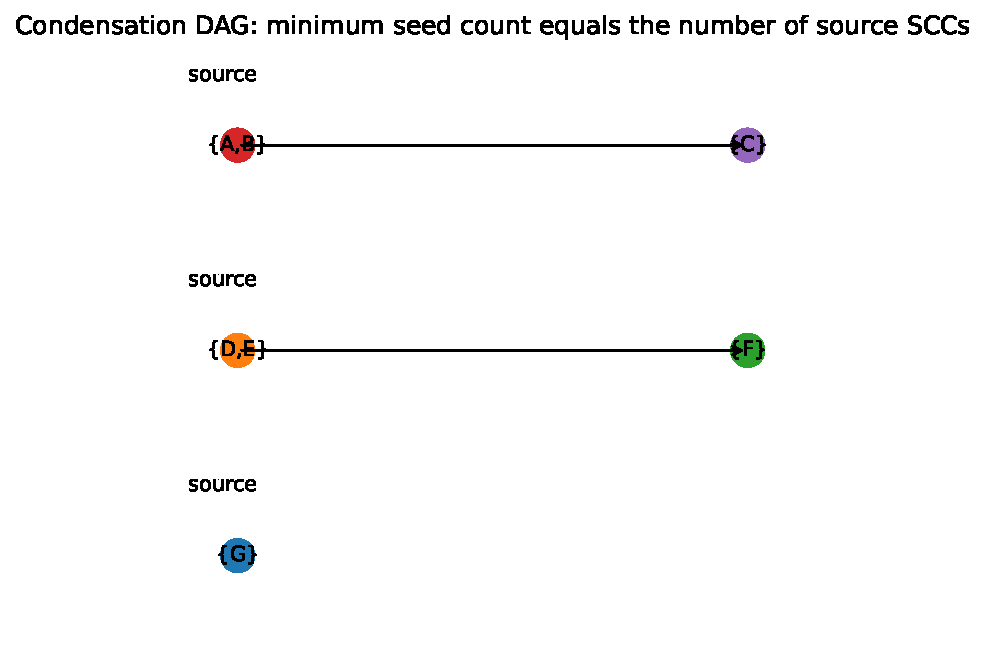
\includegraphics[width=0.86\linewidth]{10_source_scc_condensation.pdf}
\caption{The condensation DAG makes the minimum seed count visible without searching every subset of roots.}
\end{figure}

\begin{numericalcertificate}[Directed seed count]
The test graph has five strongly connected components and three source components.  The theorem gives seed rank three.  Exhaustive search over every subset of vertices independently returns three, and the selected representatives reach all seven roots.
\end{numericalcertificate}

\section{Prime-independent system seeds}

A compatible system should not be treated as an unrelated collection of \(\lambda\)-adic roots.  Its members share algebraic Frobenius polynomials, Hodge--Tate data, determinant information, and local Weil--Deligne packets.

\begin{definition}[Common arithmetic spine]
Let \(M\) be a number field.  A common spine \(\Compat\) consists of:
\begin{itemize}
\item characteristic polynomials \(P_v(X)\in M[X]\) at almost all places;
\item coefficient-prime independent weight and determinant data;
\item prescribed local Weil--Deligne or inertial packet labels at the ramified places.
\end{itemize}
For each finite place \(\lambda\) of \(M\), let
\[
X_{\lambda,m}(\Compat)
\]
be the finite set of admissible objects modulo \(\varpi_\lambda^m\) realizing the reduction of this spine.
\end{definition}

The system seed is the fibered object
\[
\boxed{
\Sys_{\mathrm{sys}}
=
\Sys_2^{\mathrm{wt}}
\times_{\Compat}
\prod_{\lambda\nmid2}'\Sys_\lambda.
}
\]
The fiber product notation states a compatibility requirement.  It does not prove that every fiber is nonempty.

\begin{theorem}[Adelic finite-depth completion]
Assume:
\begin{enumerate}
\item an algebraic common spine \(\Compat\) over a number field \(M\) is fixed;
\item for every finite place \(\lambda\) of \(M\) and every \(m\ge1\), the companion level \(X_{\lambda,m}(\Compat)\) is finite and nonempty;
\item the reduction forests are finitely branching;
\item the selected local conditions are closed under inverse limits.
\end{enumerate}
Then for every \(\lambda\) there is an infinite compatible branch
\[
\rho_\lambda\in\varprojlim_mX_{\lambda,m}(\Compat),
\]
and the collection \(\{\rho_\lambda\}_\lambda\) realizes the prescribed strictly compatible spine.
\end{theorem}

\begin{proof}
Finite-branch compactness gives an infinite branch in every coefficient-prime forest.  Inverse-limit closure gives an admissible \(\lambda\)-adic object.  By definition each finite level has the prescribed reductions of the common Frobenius and local packets.  Equality at every finite precision implies equality in the complete coefficient ring.  Thus all members realize the same spine.
\end{proof}

\begin{corollary}[Residual companion obstruction]
If
\[
X_{\lambda,1}(\Compat)=\varnothing
\]
for one coefficient prime \(\lambda\), no compatible completion with spine \(\Compat\) exists.  Deeper perturbations at other primes cannot create the missing residual companion.
\end{corollary}

\begin{figure}[H]
\centering
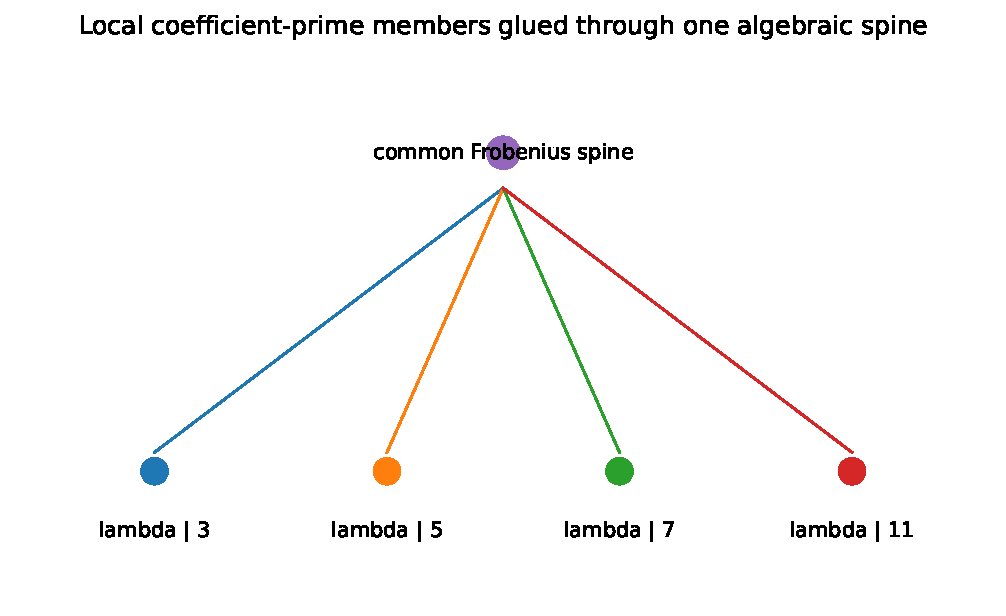
\includegraphics[width=0.82\linewidth]{13_common_system_spine.pdf}
\caption{The local members are coordinates of one system only after their finite data descend to a common algebraic spine.}
\end{figure}

\begin{example}[A scalar companion failure]
For
\[
f(x)=x^2+1,
\]
there are two simple branches at \(p=5\) and \(p=13\), no residual roots at \(p=3\) or \(p=7\), and one root modulo \(2\) that has no child modulo \(4\).  A complete \(5\)-adic branch therefore does not imply an adelic solution.
\end{example}

\begin{figure}[H]
\centering
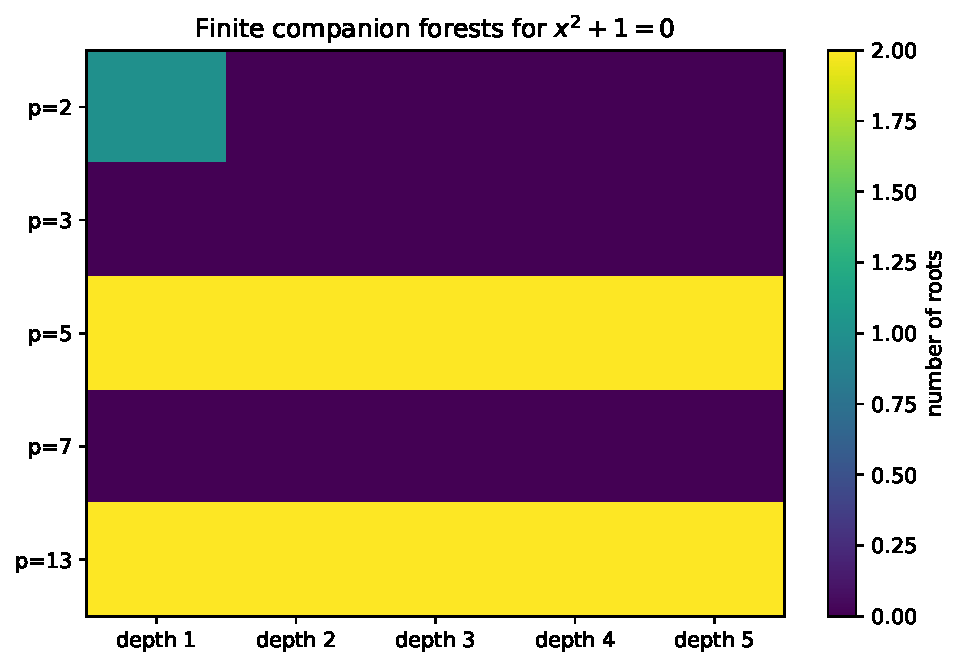
\includegraphics[width=0.79\linewidth]{12_companion_forest_occupancy.pdf}
\caption{Finite companion levels for \(x^2+1=0\).  The obstruction at \(2,3,7\) is visible before any deep lifting argument begins.}
\end{figure}

\section{Compatible carriers and finite Frobenius separation}

One useful completion mechanism is available when the desired packet already occurs as a semisimple summand of a known compatible carrier.

\begin{theorem}[Finite Frobenius separation]
Let
\[
\mathscr W_1,\ldots,\mathscr W_r
\]
be pairwise nonisomorphic strictly compatible systems whose members are absolutely irreducible.  Then there are finitely many unramified places
\[
v_1,\ldots,v_s
\]
such that the trace matrix
\[
C=
\left(
\Tr\mathscr W_{i,\lambda}(\Frob_{v_j})
\right)_{
1\le j\le s,
1\le i\le r}
\]
has column rank \(r\).  Its entries are independent of \(\lambda\).
\end{theorem}

\begin{proof}
The characters of pairwise nonisomorphic irreducible representations are linearly independent.  If all evaluation vectors on unramified Frobenius classes had rank less than \(r\), the characters would satisfy a nontrivial linear relation on a dense set and hence everywhere, a contradiction.  A finite set of evaluations witnesses the rank of a finite-dimensional function space.  Strict compatibility makes the chosen traces independent of \(\lambda\).
\end{proof}

\begin{theorem}[Compatible-carrier summand completion]
Suppose a semisimple strictly compatible carrier decomposes as
\[
\mathscr W
\cong
\bigoplus_{i=1}^{r}
\mathscr W_i^{\oplus c_i},
\]
with the \(\mathscr W_i\) as above.  At one coefficient prime \(\lambda_0\), suppose a semisimple summand has the form
\[
V_{\lambda_0}
\cong
\bigoplus_{i=1}^{r}
W_{i,\lambda_0}^{\oplus m_i},
\qquad
0\le m_i\le c_i.
\]
Then
\[
\boxed{
V_\lambda
=
\bigoplus_{i=1}^{r}
W_{i,\lambda}^{\oplus m_i}
}
\]
defines a strictly compatible summand at every coefficient prime.  The vector \((m_i)\) is uniquely recoverable from finitely many Frobenius traces supplied by the separation theorem.
\end{theorem}

\begin{proof}
Use the same multiplicities in every member of the compatible carrier.  Direct sums preserve strict compatibility, and \(m_i\le c_i\) makes \(V_\lambda\) a summand of \(W_\lambda\).  At the separating places, the target trace vector is \(C\bm m\).  Full column rank makes \(\bm m\) the unique solution.
\end{proof}

\begin{figure}[H]
\centering
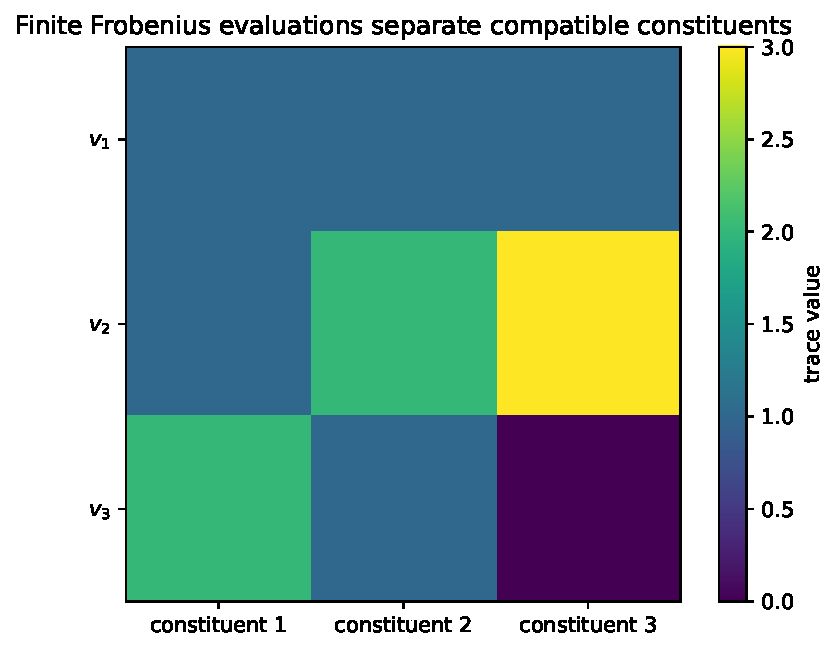
\includegraphics[width=0.72\linewidth]{14_frobenius_separator_matrix.pdf}
\caption{A finite set of trace evaluations separates three compatible constituents and recovers their multiplicities.}
\end{figure}

\begin{numericalcertificate}[Multiplicity recovery]
The exact rational solver uses three separating trace rows and reconstructs
\[
\bm m=(2,0,1)
\]
from the observed trace vector.  It rejects nonintegral solutions and multiplicities exceeding the carrier capacities.
\end{numericalcertificate}

The theorem is substantial only when a suitable compatible carrier and its irreducible compatible constituents are already known.  It does not assert that every geometric representation embeds into such a carrier.

\section{Finite spectral occupancy}

System completion produces arithmetic members.  It does not prove that a desired packet occurs in a global carrier.  In a fixed finite-dimensional semisimple carrier, however, occupancy is an exact projector question.

Let \(T_1,\ldots,T_N\) be commuting semisimple operators on a finite-dimensional vector space \(A\), and let \(a_i\) be a selected eigenvalue of \(T_i\).  Define
\[
e_i
=
\prod_{\mu\in\Spec(T_i)\setminus\{a_i\}}
\frac{T_i-\mu I}{a_i-\mu},
\qquad
e_T=\prod_{i=1}^{N}e_i,
\]
with \(e_i=0\) if \(a_i\) is absent.

\begin{theorem}[Exact finite occupancy trace]
The operator \(e_T\) is the projector onto the joint eigenspace
\[
A_T
=
\{v:T_iv=a_iv\text{ for every }i\}.
\]
Moreover,
\[
\boxed{
\Tr(e_T)=\rank(e_T)=\dim A_T\in\Z_{\ge0}.
}
\]
Thus the finite packet is occupied exactly when \(\Tr(e_T)>0\).
\end{theorem}

\begin{proof}
The Lagrange polynomial defining \(e_i\) equals one at \(a_i\) and zero at every other eigenvalue, so \(e_i\) is the spectral projector onto the selected eigenspace.  Commutativity makes their product the projector onto the intersection.  An idempotent is diagonalizable with eigenvalues zero and one, so its trace equals its rank.
\end{proof}

\begin{figure}[H]
\centering
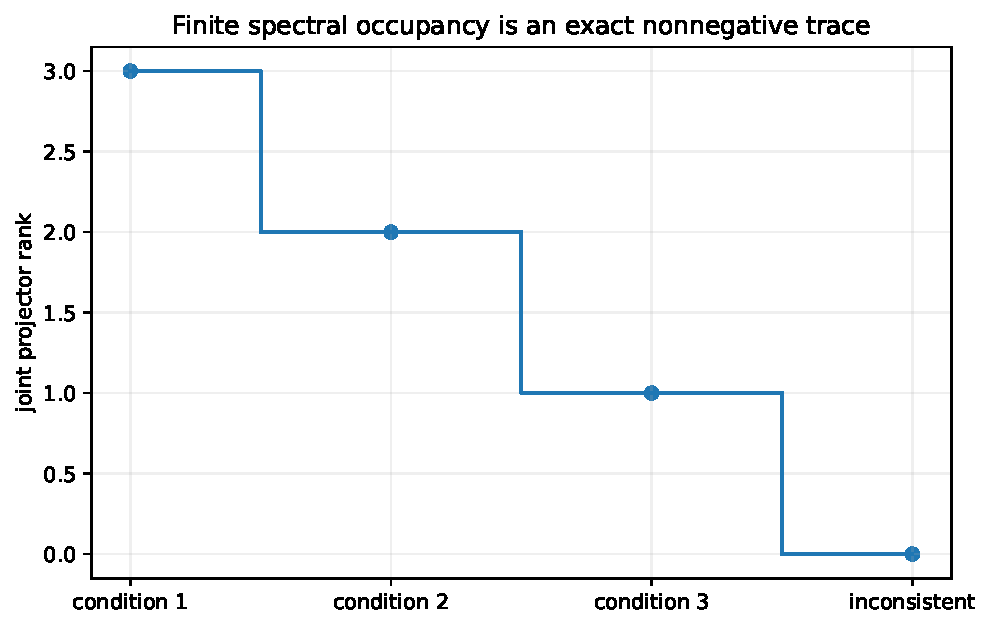
\includegraphics[width=0.77\linewidth]{15_finite_occupancy_ranks.pdf}
\caption{A consistent sequence of finite conditions narrows the carrier from ranks \(3\) to \(2\) to \(1\).  One inconsistent condition forces the joint projector to zero.}
\end{figure}

\begin{conjecture}[Universal occupancy]
For every admissible finite arithmetic packet in the intended global class, there exists a finite-dimensional carrier in which the associated joint projector has positive trace.
\end{conjecture}

This conjecture is not a consequence of the projector formula.  The formula measures occupancy exactly once the carrier is fixed.  It cannot force the trace to be positive.

\section{A conditional system-completion criterion}

The preceding results can be assembled without promoting their missing hypotheses to theorems.

\begin{theorem}[Residual-system completion criterion]
Fix an admissible arithmetic class.  Suppose:
\begin{enumerate}
\item every object has a unique residual root in an exhaustive residual moduli space;
\item a common algebraic spine is defined for the desired system;
\item every coefficient-prime residual companion exists;
\item every companion forest has nonempty finite levels, finite branching, and inverse-limit closed local conditions;
\item the required horizontal transports preserve the common spine and the selected local deformation conditions.
\end{enumerate}
Then the desired strictly compatible arithmetic system exists.  If, in addition, the system is a summand of a known compatible carrier, the summand is recovered at every coefficient prime by finitely many Frobenius traces.
\end{theorem}

\begin{proof}
The first four hypotheses give the system by adelic finite-depth completion.  The transport hypothesis identifies any roots that are meant to be generated horizontally without changing the prescribed spine.  The final assertion is the compatible-carrier summand theorem.
\end{proof}

\begin{corollary}[Exact location of the remaining existence problem]
After vertical completeness has been established, the remaining system problem is horizontal:
\[
\boxed{
\begin{aligned}
\text{companion existence: }&X_{\lambda,1}(\Compat)\ne\varnothing
\text{ for every }\lambda;\\
\text{finite occupancy: }&\Tr(e_T)>0
\text{ for every required global packet.}
\end{aligned}}
\]
Neither statement is created by increasing the perturbation depth above an already existing root.
\end{corollary}

\begin{conjecture}[Natural finite seed rank]
For the admissible residual transport category attached to a fixed arithmetic class, the directed seed rank is finite.  A one-seed theorem is the stronger assertion that the condensation category has exactly one source component and that all required transports preserve deformation and occupancy data.
\end{conjecture}

\section{Worked finite models}

\subsection{Smooth branch}

For \(q=3\) and formal dimension \(d=2\), the finite levels have cardinalities
\[
1,9,81,729,6561,\ldots.
\]
The seed zeta function is
\[
Z(T)=\frac{T}{1-9T}.
\]

\subsection{Weighted dyadic chart}

For weights \((1,2,4)\), the counts are
\[
1,2,8,32,256,2048,\ldots.
\]
The first coordinate is active immediately, the second one level later, and the third at depth five.  The exact rational function generated by the code is
\[
Z_{(1,2,4)}(T)
=
\frac{T(1-6T-8T^2-32T^3)}{1-8T}.
\]
The negative signs in this presentation arise from moving the denominator to \(1-8T\); every power-series coefficient is positive.

\subsection{Singular branch}

For \(x^2=0\) over a residue field of size three, the counts are
\[
1,3,3,9,9,27,27,81,\ldots,
\]
and
\[
Z(T)=\frac{T+3T^2}{1-3T^2}.
\]
The exact branching dimension is \(1/2\).

\subsection{Directed transport}

The finite graph in \cref{fig:transport-graph} has three source components.  The source-component theorem and brute-force enumeration both return the minimum seed count three.

\begin{figure}[H]
\centering
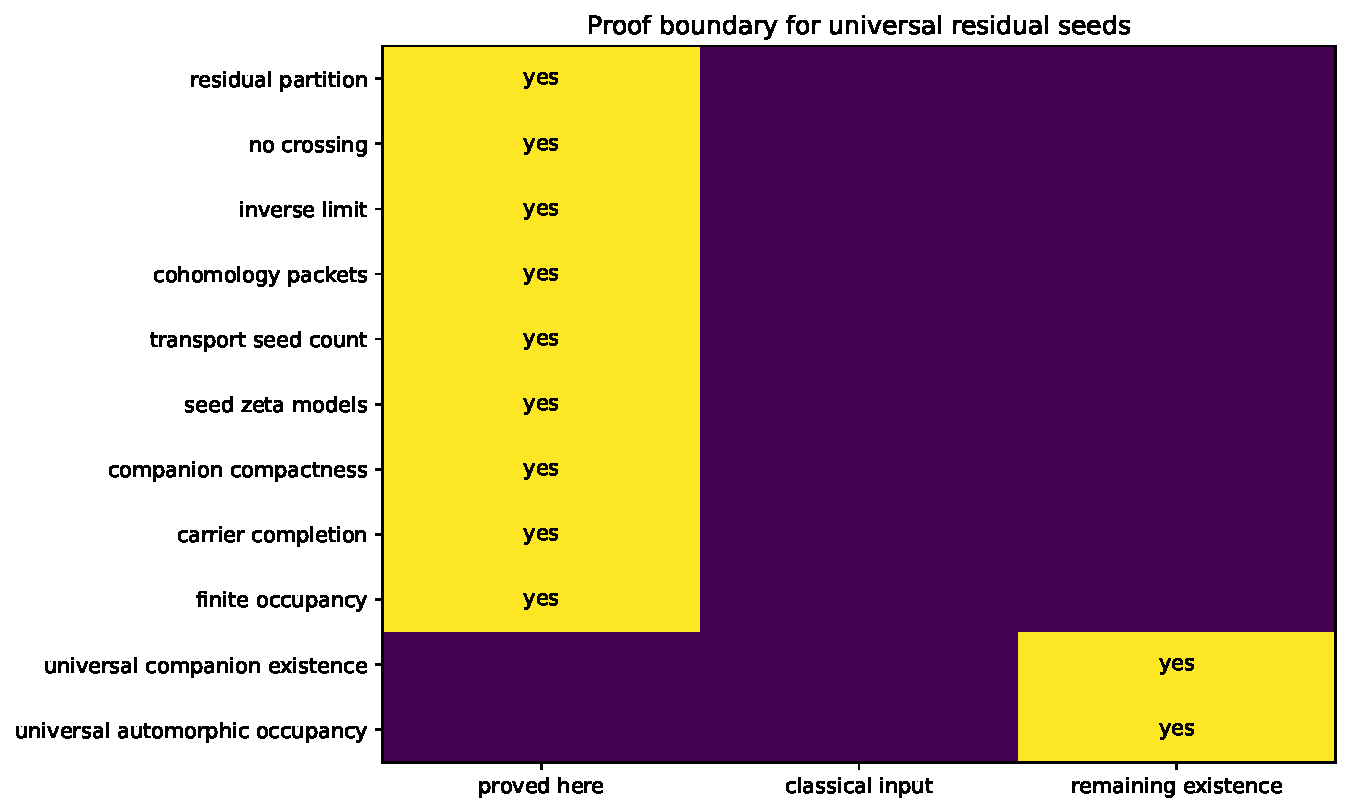
\includegraphics[width=0.84\linewidth]{16_proof_status.pdf}
\caption{The finite and formal statements proved in this paper are separated from the two remaining universal existence assertions.}
\label{fig:proof-status}
\end{figure}

\section{Computational certificates}

The code uses exact integer, rational, symbolic, and modular arithmetic for all mathematical identities.  Floating-point arithmetic is used only to render the figures and to report a regression estimate alongside an exact branching dimension.

\begin{table}[H]
\centering
\caption{Selected exact certificates.}
\begin{tabular}{lr}
\toprule
Certificate & Result\\
\midrule
Residual packet count in the mod-three model & 3\\
Compatible base-five inverse-limit branch & yes\\
First dyadic sign separation depth & 2\\
Source strongly connected components & 3\\
Brute-force minimum directed seed count & 3\\
Cohomology packet reconstruction residual & 0\\
Compatible common-spine test & passed\\
Inconsistent spine detected & yes\\
Recovered carrier multiplicities & \((2,0,1)\)\\
Finite occupancy ranks & \((3,2,1,0)\)\\
\bottomrule
\end{tabular}
\end{table}

The complete automated suite contains \(28\) tests.  They cover residual partition, no crossing, inverse-limit digits, weighted and singular zeta coefficients, directed source components, cohomology packets, companion forests, common-spine consistency, finite Frobenius separation, multiplicity recovery, and exact occupancy projectors.

\section{Claim ledger}

\begin{longtable}{p{0.34\linewidth}p{0.18\linewidth}p{0.40\linewidth}}
\toprule
Statement & Status & Scope or boundary\\
\midrule
\endfirsthead
\toprule
Statement & Status & Scope or boundary\\
\midrule
\endhead
Residual partition & proved & any moduli functor with well-defined reduction\\
No crossing & proved & operations trivial at residual depth\\
Inverse-limit reconstruction & proved & represented complete deformation problem\\
Finite-branch compactness & proved & finite nonempty levels and finite branching\\
Smooth and weighted seed zeta formulas & proved & stated formal coordinate models\\
Singular power zeta and dimension & proved & scalar equation \(x^e=0\)\\
Cohomology packet decomposition & proved & chain projectors commuting with the differential\\
Directed minimum-seed theorem & proved & finite directed transport graph\\
Adelic finite-depth completion & proved & common spine, all finite levels occupied, closed local conditions\\
Compatible-carrier summand completion & proved & known semisimple compatible carrier and finite separation\\
Finite occupancy trace & proved & fixed finite-dimensional semisimple commuting carrier\\
Universal residual companions & not proved & requires nonempty root at every coefficient prime\\
Universal compatible-system completion & not proved & algebraic spine and companion occupancy remain necessary\\
Universal automorphic occupancy & not proved & requires positive global packet traces\\
Unrestricted reciprocity & not claimed & belongs to later local and global papers\\
\bottomrule
\end{longtable}

\section{Conclusion}

The residual seed theory becomes precise once vertical and horizontal generation are separated.  Positive-depth perturbations can be complete within one formal component.  They cannot change the residual root.  The universal arithmetic seed is therefore a forest rather than one branch:
\[
\boxed{
\text{residual roots}
\longrightarrow
\text{finite deformation levels}
\longrightarrow
\text{inverse-limit branches}.
}
\]

Projectors add three useful structures to this forest.  They split tangent and obstruction complexes into exact subproblems, they measure delayed dyadic visibility through weights, and they turn finite carrier occupancy into an integer trace.  Directed transport adds a fourth: it converts the informal question ``how many seeds are needed?'' into the source-component count of a condensation graph.

The system-level boundary is now narrow enough to state without ambiguity.  One must construct a common algebraic spine, populate every residual companion forest, lift those companions through all depths, and prove positive occupancy of the required global packets.  The present paper proves the formal reconstruction, counting, transport, compactness, carrier, and finite-projector theorems used in that reduction.  It does not assert the missing universal existence statements.

\appendix

\section{Algorithms implemented in the companion package}

\subsection{Residual towers}

The residual module partitions coordinates modulo \(p\), verifies compatibility
\[
x_{m+1}\equiv x_m\pmod{p^m},
\]
and reconstructs the digit \(a_{m-1}\) by
\[
a_{m-1}=\frac{x_m}{p^{m-1}}\pmod p.
\]

\subsection{Transport condensation}

The transport module computes strongly connected components by two depth-first passes, forms the condensation graph, finds all source components, and selects one representative from each.  A brute-force subset search is included only as an independent finite certificate.

\subsection{Companion forests}

For an integral polynomial \(f\), the finite root forest is obtained by exact enumeration of
\[
f(x)\equiv0\pmod{p^m}
\]
and by connecting a child \(x_{m+1}\) to its reduction modulo \(p^m\).  This is intended for small exact examples, not large deformation rings.

\subsection{Cohomology packets}

Modular Gaussian elimination computes the ranks of the differentials.  For
\[
C^{i-1}\xrightarrow{d_{i-1}}C^i\xrightarrow{d_i}C^{i+1},
\]
the finite dimension is evaluated as
\[
\dim H^i
=
\dim C^i-\rank d_i-\rank d_{i-1}.
\]
Packet subcomplexes are computed separately and checked against the total.

\subsection{Finite occupancy}

For each commuting semisimple operator, a Lagrange polynomial constructs the exact spectral idempotent.  Their product gives the joint packet projector.  Symbolic rational arithmetic verifies idempotence and the equality of trace and rank.

\section{Reproducibility boundary}

The companion code is a finite certificate library.  It does not construct universal Galois deformation rings, compute general continuous group cohomology, prove representability, discover compatible systems, or evaluate automorphic trace formulas.  Those are mathematical inputs or later existence problems.  The release is designed to make every finite example and every displayed count independently reproducible without confusing computation with proof.

\end{document}
